
\section{Image Calibration}
\label{sec:image-calibration}

The first step in the analysis is to preprocess the raw images to correct for various
sources of noise. This is necessary for the star identification, magnitude estimation and
other analyses the user might want to perform to give accurate results. In this section,
all steps of the preprocessing pipeline are described in detail. First, the observations
that I used for testing are described in \autoref{sec:observations}. Reading the raw image
data is covered in \autoref{sec:raw-image-data}. The subsequent processing steps are pixel
correction (\autoref{sec:faulty-pixels}), vignetting correction
(\autoref{sec:vignetting-correction}), interpolation (\autoref{sec:interpolation}) and
skyglow correction (\autoref{sec:skyglow-correction}). Finally, the full pipeline with
some minor additional processing steps is described in \autoref{sec:full-pipeline}.

\subsection{Observations}
\label{sec:observations}

To test my processing pipeline and perform the analysis, I used a set of wide-field images
photographed with a Canon EOS 1200D camera and a 18-55 mm lens, mounted on a tripod. The
images were taken in the Stadtpark in Aachen and under good weather conditions. Even
though images taken under perfect conditions would be ideal for estimating the
source-count distribution, they would not be ideal for testing the robustness of the
methods. The pipeline is able to handle different types of noise and bias, like faulty
pixels (\autoref{sec:faulty-pixels}) and skyglow (\autoref{sec:skyglow-correction}). I
selected the best image and used it for the analysis to keep the results comparable. The
camera settings for this image are shown in \autoref{tab:camera-settings}. In general, I
varied the exposure time and ISO settings to capture images with different levels of
brightness and noise. All images were taken with an aperture of f/3.5 and a focal length
of 18 mm and were saved in the Canon CR2 raw image format. An example image is shown in
\autoref{fig:sky-input}.

\begin{table}[tb]
  \centering
  \begin{tabular}{ll}
    \toprule
    \textbf{Parameter} & \textbf{Value}        \\
    \midrule
    Sensor size        & $22.3 \times 14.9$ mm \\
    Image resolution   & $5202 \times 3465$ px \\
    Bit depth          & 14 bits               \\
    Aperture           & f/3.5                 \\
    Focal length       & 18 mm                 \\
    Exposure time      & 10 s                  \\
    ISO                & 6400                  \\
    \bottomrule
  \end{tabular}
  \caption{Camera specifications and settings for the night sky image used throughout this paper.}
  \label{tab:camera-settings}
\end{table}

\begin{figure}[tb]
  \centering
  \begin{subfigure}{.45\textwidth}
    \centering
    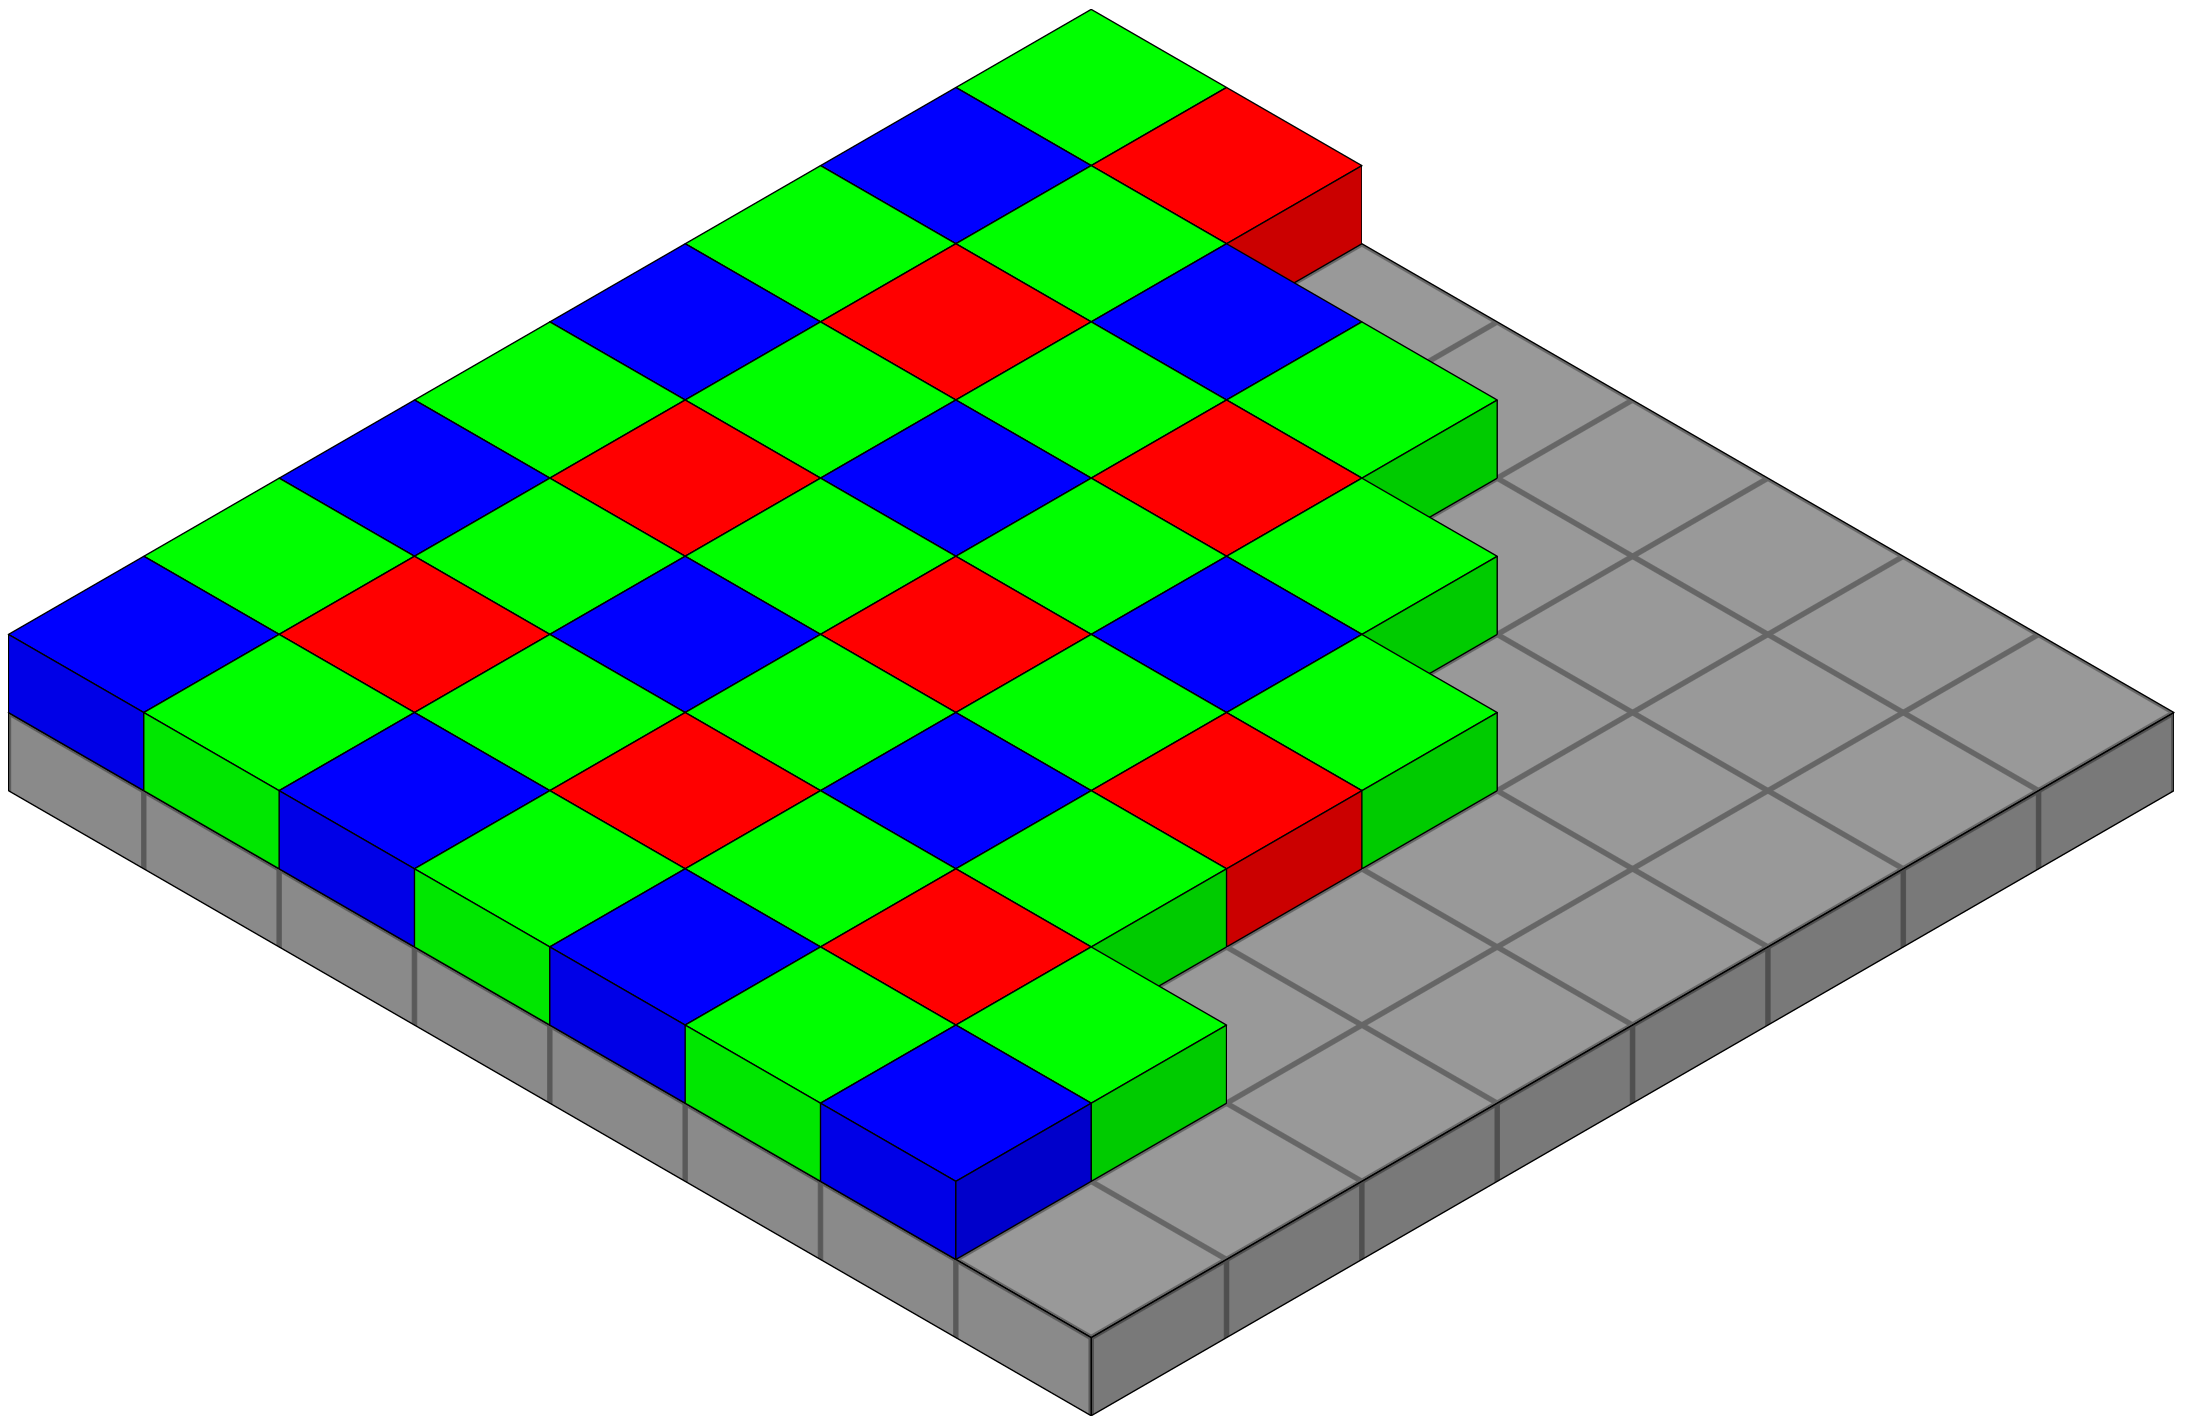
\includegraphics[width=.8\linewidth]{bayer-pattern.png}
    \caption{An example Bayer arrangement of color filters on the pixel array of an image sensor.}
    \label{fig:bayer-pattern}
  \end{subfigure}%
  \hfill
  \begin{subfigure}{.45\textwidth}
    \centering
    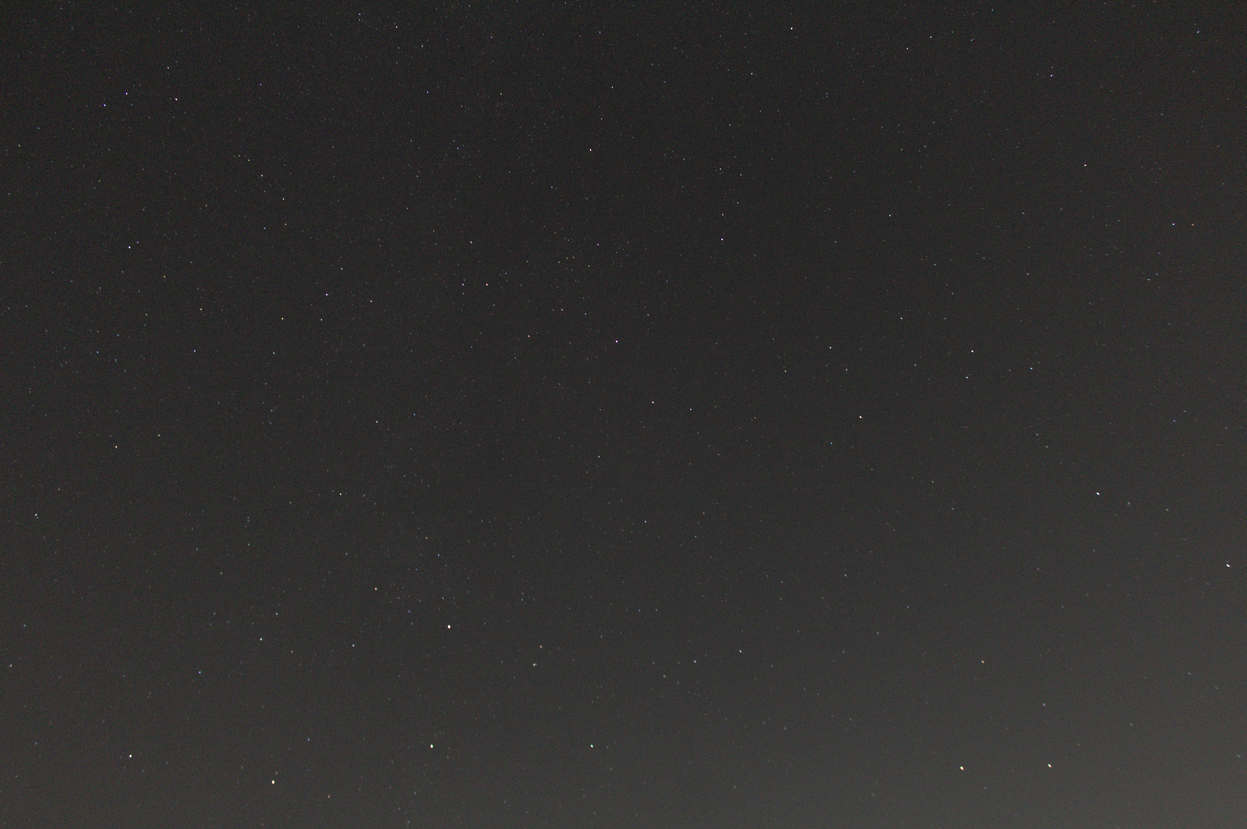
\includegraphics[width=\linewidth]{sky-input.png}
    \caption{The night sky image used throughout this paper, converted from raw to RGB.}
    \label{fig:sky-input}
  \end{subfigure}
  \caption{}
\end{figure}

In addition to the night sky images, I also took black and white field images for
calibration. The black images were taken with the lens cap on, before and after each set
of night sky images, to match the conditions of the night sky images as closely as
possible. The white images were taken out of focus, with a homogeneously illuminated white
paper covering the entire field of view. To avoid saturation of the sensor, the shutter
speed for the white images was set to 5 ms. The black images were used to reduce the noise
in dark pixels (\autoref{sec:full-pipeline}), while the white images were used to correct
for vignetting (\autoref{sec:vignetting-correction}).

\subsection{Raw Image Data}
\label{sec:raw-image-data}

Raw images store the unprocessed data captured by the camera sensor without any
modifications. For the Canon EOS 1200D, this is a matrix with values ranging from 0 to
16383, representing the intensity of light captured. Each pixel has a red, green or blue
color filter, corresponding to the Bayer pattern used by the camera. An example of a Bayer
arrangement is shown in \autoref{fig:bayer-pattern}. The camera that I used has the
following pattern:
\begin{align*}
  \begin{bmatrix}
    R & G \\
    G & B \\
  \end{bmatrix}
\end{align*}
This pattern is repeated for each $2 \times 2$ pixel block in the image. For my analysis,
I am only interested in the intensity of light, instead of the color. As 50\% of the
pixels in the image are green, I only use the green channel for further processing. All
methods of my software library can be used equally with the red and blue channels, but
this will not be discussed in this paper. I masked the red and blue pixels, which leaves a
checkerboard pattern of green pixels, as shown in \autoref{fig:faulty-pixels}. The missing
pixels will be filled in using interpolation (\autoref{sec:interpolation}), because the
methods from the OpenCV library require a complete image. However, it is important to
interpolate at the latest possible stage, to avoid introducing artifacts and additional
bias into the image. I used the \texttt{rawkit} library \cite{rawkit2025} to read the raw
images, which is a Python wrapper for the LibRaw library and also provides metadata about
the images.

I selected a night sky image with a high number of stars and a low level of noise to test
the processing pipeline and perform the analysis. The image was taken with an exposure
time of 10 s and an ISO setting of 6400 and is shown in \autoref{fig:sky-input}. In the
following sections, I will refer to this image with the red and blue channels masked as
the \textit{input image}.

\subsection{Faulty Pixels}
\label{sec:faulty-pixels}

\begin{figure}[tb]
  \centering
  \begin{subfigure}{.49\textwidth}
    \centering
    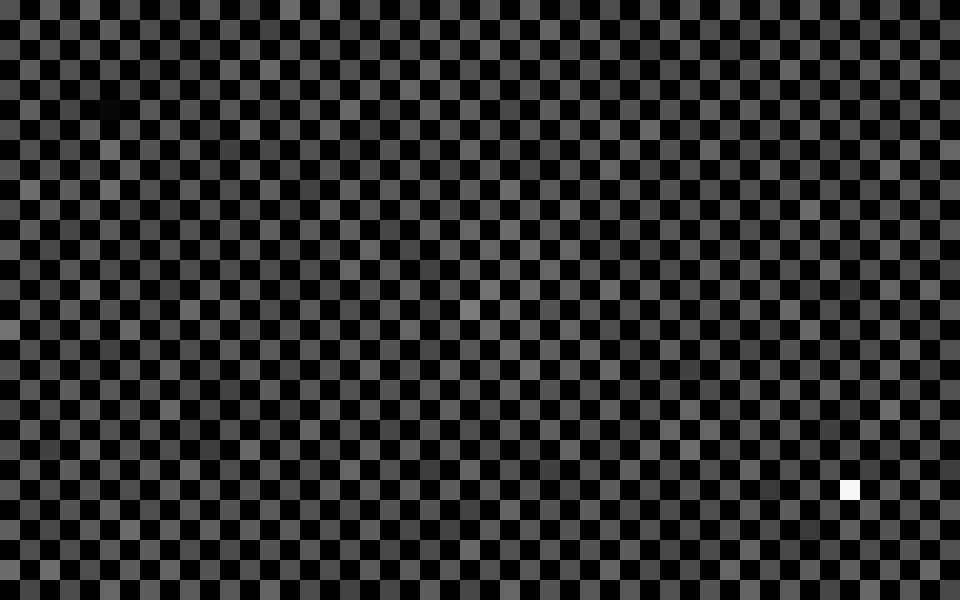
\includegraphics[width=\linewidth]{faulty-before.png}
    \caption{Before correction}
    \label{fig:faulty-before}
  \end{subfigure}%
  \hfill
  \begin{subfigure}{.49\textwidth}
    \centering
    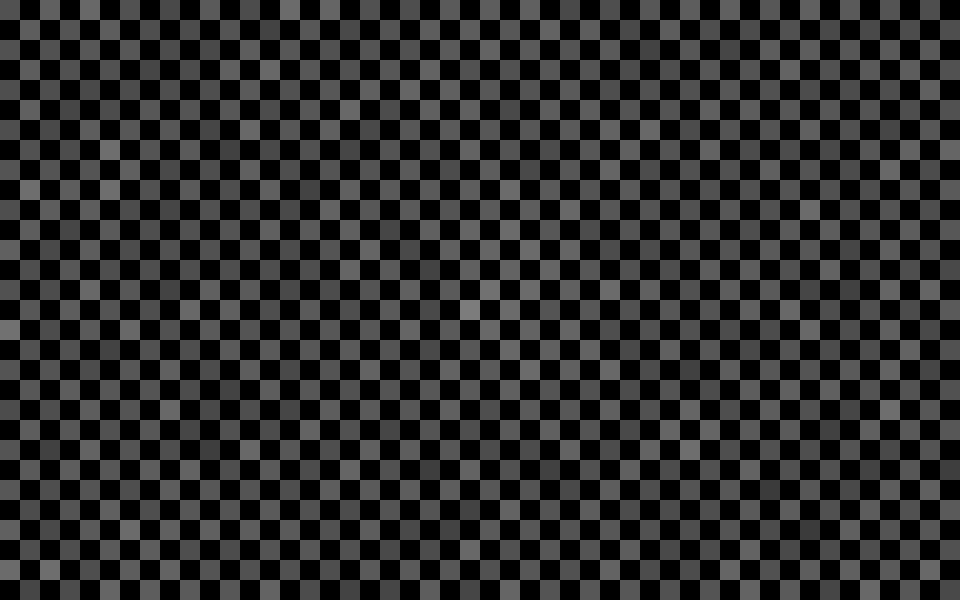
\includegraphics[width=\linewidth]{faulty-after.png}
    \caption{After correction}
    \label{fig:faulty-after}
  \end{subfigure}
  \caption{A cutout of the input image with a dead pixel in the top left and a hot pixel
    in the bottom right, before and after applying the method described in
    \autoref{sec:faulty-pixels}.}
  \label{fig:faulty-pixels}
\end{figure}

A pixel is considered faulty if it does not respond to light as expected. This needs to be
corrected before further analysis, as it can reduce the accuracy of finding stars or
predicting their magnitudes. I considered two types of faulty pixels. First, a pixel can
be permanently damaged due to a malfunction in the sensor, which can cause it to have an
incorrect sensitivity to light. Second, a pixel can be faulty due to cosmic rays or other
sources of radiation, which can cause it to receive more light than expected. Both types
result in a pixel that has a higher or lower intensity than its neighbors.

To identify faulty pixels, I compared each pixel to its neighbors in the night sky input
image. Let $I \in \mathbb{R}^{m \times n}$ be the input image and $I_{ij}$ be the
intensity of pixel $(i,j)$. I define the convolution kernel $K \in \mathbb{R}^{3 \times
    3}$ as
\begin{align*}
  K = \frac{1}{4} \begin{bmatrix}
                    1 & 0 & 1 \\
                    0 & 0 & 0 \\
                    1 & 0 & 1
                  \end{bmatrix}.
\end{align*}
Then, the mean and the standard deviation of the neighboring pixels are given by
\begin{align*}
  \mu(I)    & = I \ast K,                       \\
  \sigma(I) & = \sqrt{\mu(I^{2}) - \mu(I)^{2}},
\end{align*}
where $\ast$ denotes the convolution operation. Let $t_{\text{hot}}$ and $t_{\text{dead}}$
be thresholds for hot and dead pixels, respectively. A pixel $(i,j)$ is considered hot if
\begin{align*}
  I_{ij} > \mu(I)_{ij} + t_{\text{hot}} \cdot \sigma(I)_{ij},
\end{align*}
and dead if
\begin{align*}
  I_{ij} < \mu(I)_{ij} - t_{\text{dead}} \cdot \sigma(I)_{ij}.
\end{align*}
The thresholds can be set by the user. In my analysis, I set $t_{\text{hot}} = 3$ and
$t_{\text{dead}} = 1.2$. I chose these values by visually inspecting the images to verify
that the method correctly identifies pixels that I would consider faulty. For the input
image, this method identified 42 hot pixels and 107 dead pixels. The detected pixels are
replaced by the mean of the neighboring pixels. An example of the correction of a dead and
a hot pixel is shown in \autoref{fig:faulty-pixels}.

An alternative approach to identifying the first type of faulty pixels is to recognize
bright pixels in the black images and dark pixels in the white images. However, as can be
seen in the white image histogram in \autoref{fig:vignette-histogram} and the black image
histogram in \autoref{fig:black-histogram}, my camera did not have any permanently damaged
pixels, so I could not test this method. Also, the method described above should be able
to identify both types of faulty pixels. Therefore, I did not implement this alternative
approach.


\subsection{Vignetting Correction}
\label{sec:vignetting-correction}

As light rays from the edges of the lens have to travel a longer distance to reach the
sensor, the intensity of light is lower at the edges of the image. This effect is called
vignetting and can be corrected by dividing the input image by the white field image.
Because the white field image is homogeneously illuminated, the vignetting effect is the
main feature of the image. The white field image is shown in \autoref{fig:vignette-photo},
and its green channel histogram is shown in \autoref{fig:vignette-histogram}. It is
important that the brightest pixels are not saturated to cover the full range of
intensities. We need to normalize the white field image, as the center of the vignette
should correspond to a correction factor of 1 and the mean and standard deviation of the
distribution depend on camera settings, like the exposure time. Therefore, we divide the
white image by its 99.999th percentile, which, in this case, corresponds to the 18025th
brightest pixel. This is similar to the maximum, but more robust to outliers.

\begin{figure}[htbp]
  \centering
  \begin{subfigure}{.49\textwidth}
    \centering
    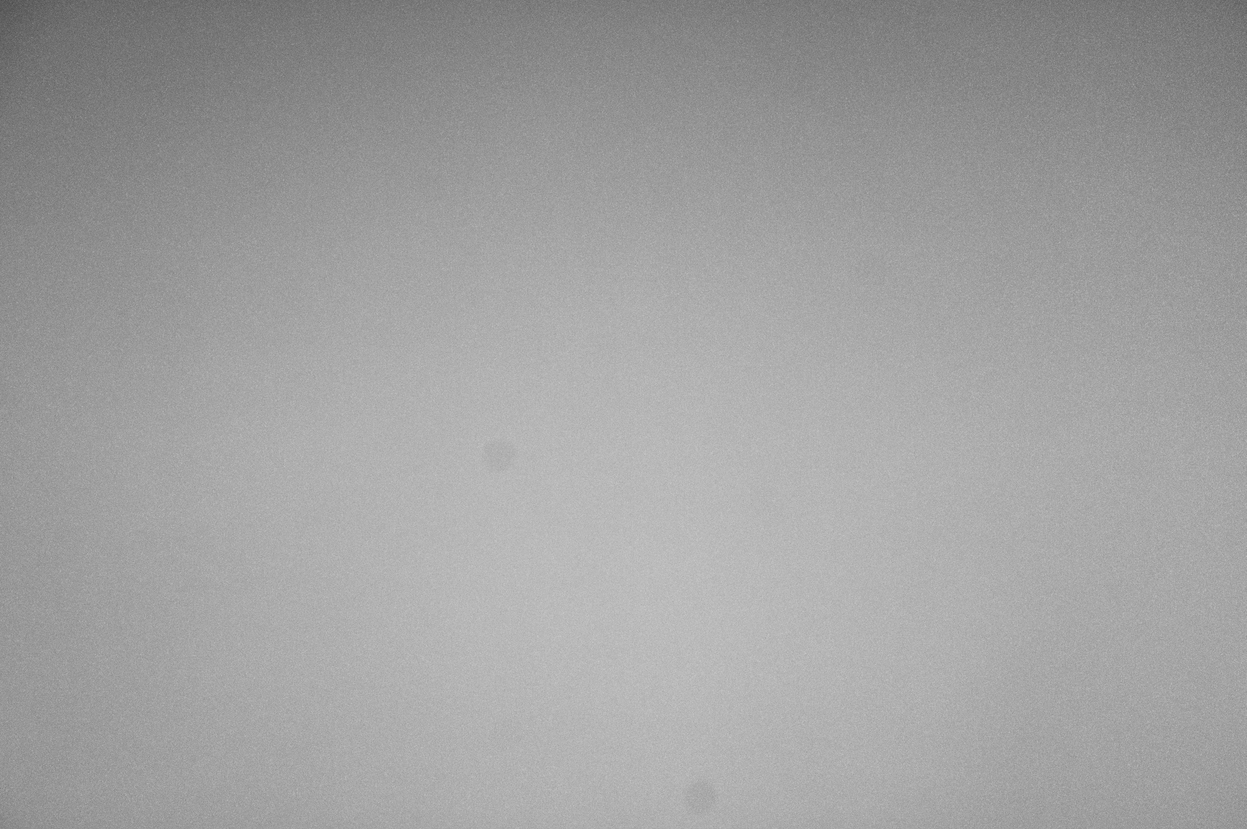
\includegraphics[width=\linewidth]{vignette-photo.png}
    \caption{The white field image with reduced brightness and increased contrast for better visualization.}
    \label{fig:vignette-photo}
  \end{subfigure}%
  \hfill
  \begin{subfigure}{.49\textwidth}
    \centering
    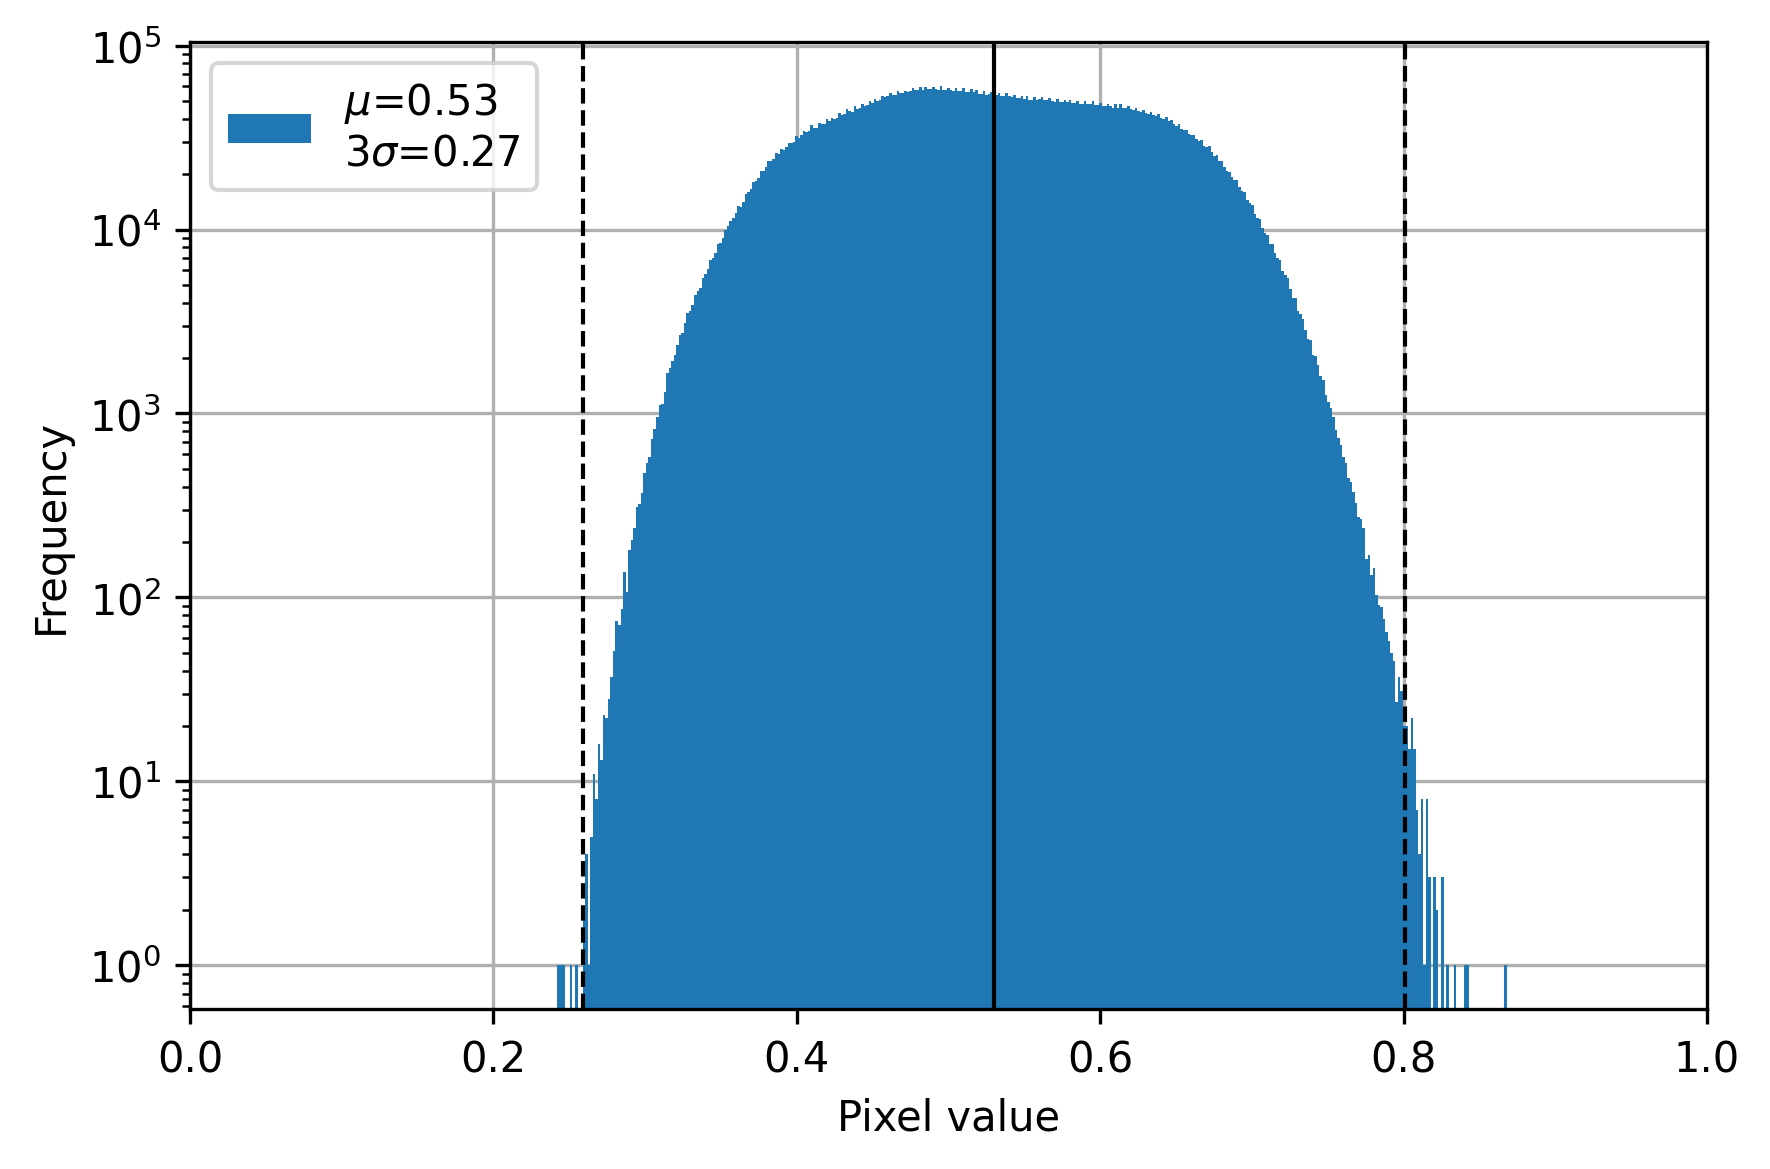
\includegraphics[width=\linewidth]{vignette-histogram.png}
    \caption{Histogram of the green channel of the white field image with relative pixel values.}
    \label{fig:vignette-histogram}
  \end{subfigure}
  \caption{}
\end{figure}

Finally, we divide the input image by the normalized white field image. The result is
shown in \autoref{fig:vignette-correction}. The vignetting effect is subtle, but visible.
In particular, the light pollution is now more pronounced in the bottom right corner,
because it was previously masked by the vignetting. I noticed that the white field image
has multiple dark spots, which are also visible in the input image, if the contrast is
increased. I cleaned the lens on the inside and outside and the mirror of the camera, but
the spots remained. I suspect that they are caused by dust on a lens element inside the
camera, which is difficult to clean without professional equipment. However, dividing by
the white field image also corrects for these spots.

\begin{figure}[htbp]
  \centering
  \begin{subfigure}{.49\textwidth}
    \centering
    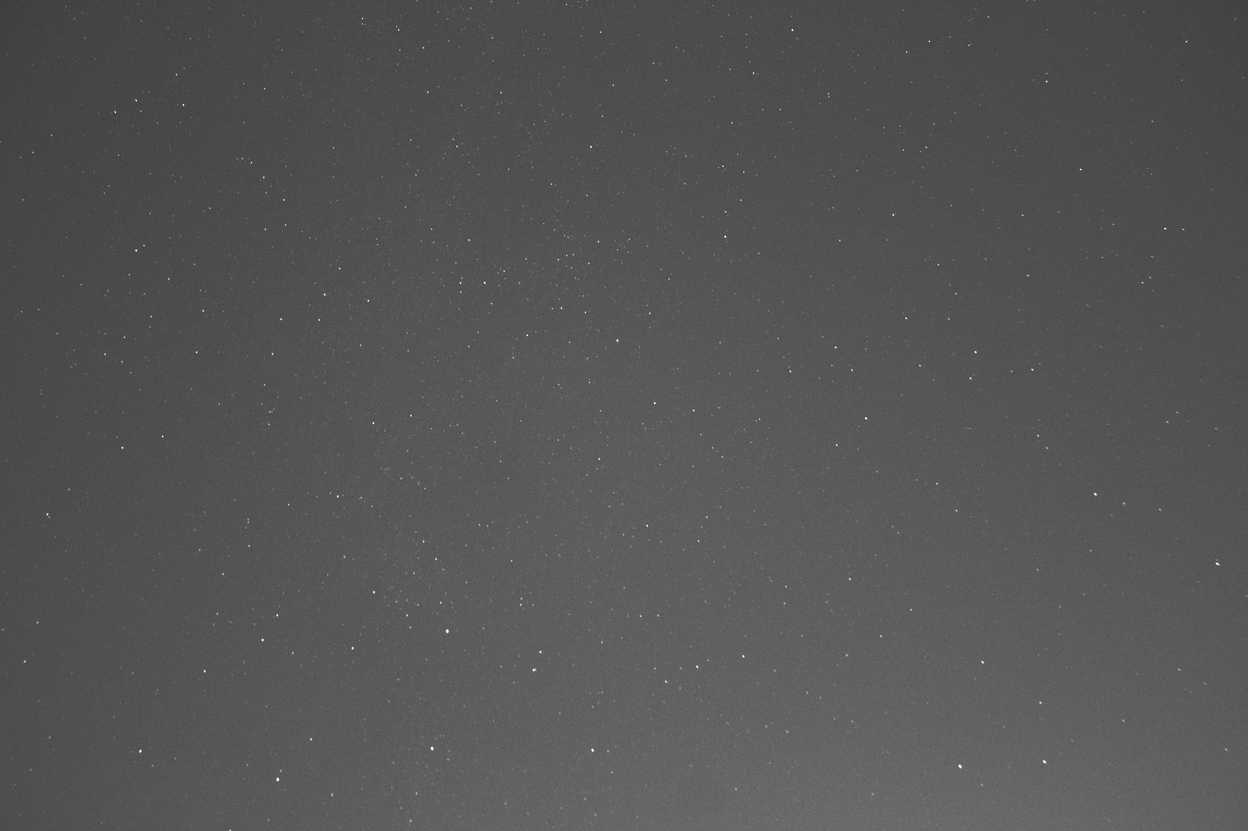
\includegraphics[width=\linewidth]{sky_green_interpolated.png}
    \caption{Before vignetting correction}
  \end{subfigure}%
  \hfill
  \begin{subfigure}{.49\textwidth}
    \centering
    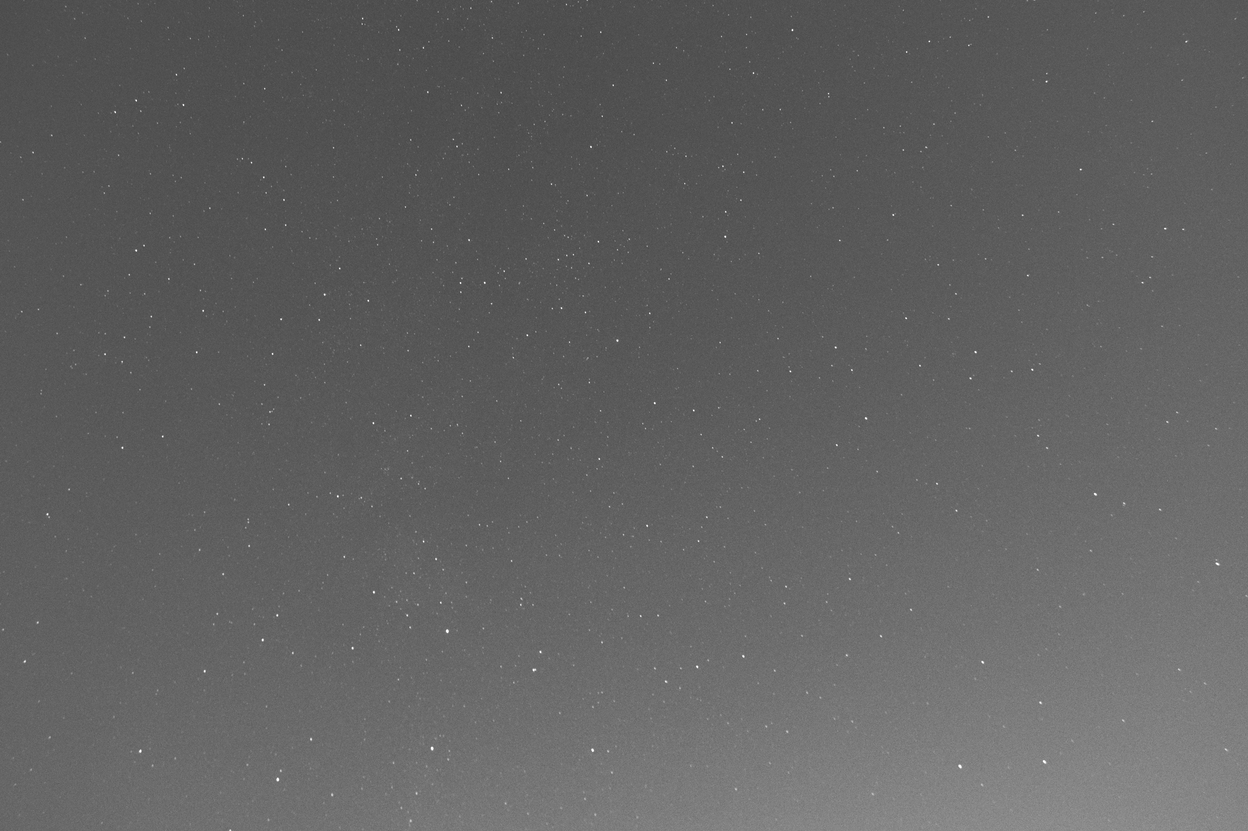
\includegraphics[width=\linewidth]{vignette_corrected.png}
    \caption{After vignetting correction}
  \end{subfigure}
  \caption{The input image before and after applying the method described in
    \autoref{sec:vignetting-correction}, interpolated for better visualization, as
    described in \autoref{sec:interpolation}.}
  \label{fig:vignette-correction}
\end{figure}

\subsection{Interpolation}
\label{sec:interpolation}

As the next steps in the pipeline require a complete image, we need to interpolate the
missing pixels. Iterating over the pixels separately would take several seconds for an
image of this size, so I used a convolution with the following kernel instead.
\begin{align*}
  K = \frac{1}{4} \begin{bmatrix}
                    0 & 1 & 0 \\
                    1 & 0 & 1 \\
                    0 & 1 & 0
                  \end{bmatrix}.
\end{align*}
Each missing pixel is replaced by the corresponding pixel in the convolution of the input
image with the kernel. The result is shown in \autoref{fig:interpolation}.

\begin{figure}[tb]
  \centering
  \begin{subfigure}{.33\textwidth}
    \centering
    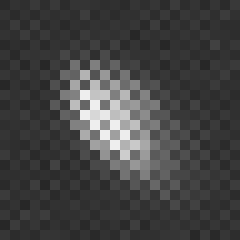
\includegraphics[width=\linewidth]{raw_cutout.png}
    \caption{Raw image}
  \end{subfigure}%
  \hfill
  \begin{subfigure}{.33\textwidth}
    \centering
    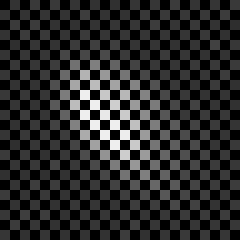
\includegraphics[width=\linewidth]{green_only_cutout.png}
    \caption{After masking}
  \end{subfigure}%
  \hfill
  \begin{subfigure}{.33\textwidth}
    \centering
    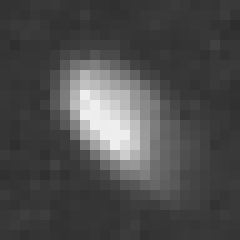
\includegraphics[width=\linewidth]{green_interpolated_cutout.png}
    \caption{After interpolation}
  \end{subfigure}
  \caption{A cutout of the input image, comparing it at different stages of the pipeline.}
  \label{fig:interpolation}
\end{figure}


\subsection{Skyglow Correction}
\label{sec:skyglow-correction}

Another common source of noise in night sky images is light pollution from artificial
sources, like street lamps or buildings. This light is reflected by particles in the
atmosphere and causes a bright background in the image. I refer to this effect as skyglow.
It appears as a smooth gradient in the image with no hard edges or localized features.
Stars, on the other hand, are point sources of light and have a sharp intensity profile.
Therefore, we can correct for skyglow by subtracting a smoothed version of the image from
the original image.

To smooth the image, I used a Gaussian filter with a kernel size of $700 \times 700$
pixels and a standard deviation of 200 pixels. The kernel size is chosen to be large, so
that all stars are fully smoothed out. The smoothed image is shifted by subtracting its
minimum pixel value to avoid negative values. The corrected image is then obtained by
subtracting the smoothed image from the input image and clipping the result to the range
$[0, 16383]$.

The blurred image and the result of the skyglow correction are shown in
\autoref{fig:skyglow}. The gradient in the blurred image shows lines instead of a smooth
gradient. This is because the original blurred image is very dim and, to show it in this
paper, I converted it to 8-bit and increased the contrast and brightness. As the original
image is 14-bit, the lines are not visible there. After correction, the background of the
processed image is much more uniform. However, this method is only beneficial for
wide-field images with no obstructing objects. If there are trees, buildings or the moon
in the image, subtracting the blurred image might worsen the magnitude estimation near the
objects. Also, in images with a narrow field of view, the skyglow is much more uniform,
making the method unnecessary. The user can disable the skyglow correction in these cases.

\begin{figure}[tb]
  \centering
  \begin{subfigure}{.49\textwidth}
    \centering
    
\includegraphics[width=\linewidth]{skyglow_blurred.png}
    \caption{Input image after blurring, adjusted for better visualization.}
    \label{fig:skyglow-blurred}
  \end{subfigure}%
  \hfill
  \begin{subfigure}{.49\textwidth}
    \centering
    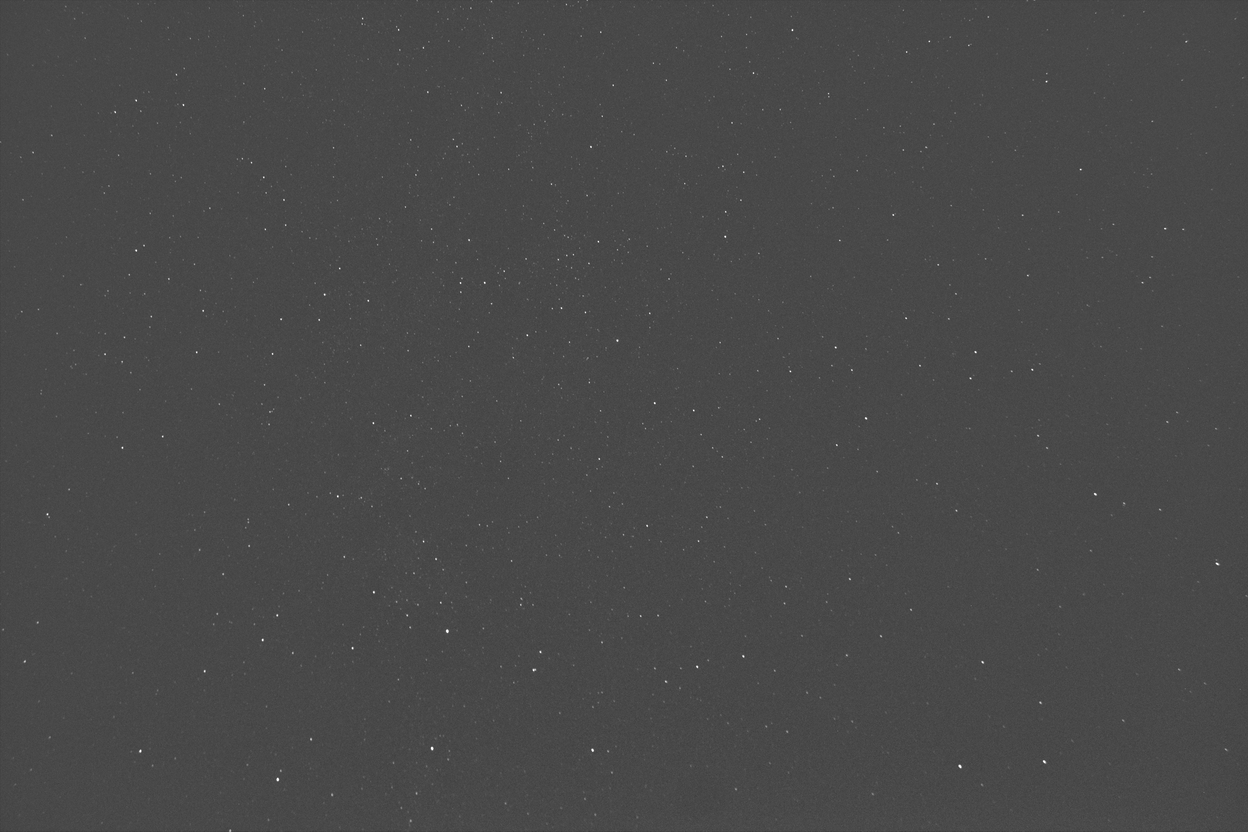
\includegraphics[width=\linewidth]{skyglow_corrected.png}
    \caption{The processed image after skyglow correction.\\\text{}}
    \label{fig:skyglow-corrected}
  \end{subfigure}
  \caption{Skyglow correction, see \autoref{sec:skyglow-correction}}
  \label{fig:skyglow}
\end{figure}

\subsection{Full Pre-Processing Pipeline}
\label{sec:full-pipeline}

The previous sections describe the major steps of the pre-processing pipeline. An overview
of the order of the steps and how they are applied to the input image is shown in
\autoref{fig:full-pipeline}. The pipeline takes a raw night sky image, a black field image
and a white field image as input. The red and blue channels of all images are masked (not
shown in the figure for simplicity). After the faulty pixels are corrected, the mean of
the black image is subtracted from the input image and the result is clipped to the range
$[0, 16383]$. This reduces the noise in the dark pixels because every pixel with a value
below the mean of the black image is set to 0. The next steps are the vignetting
correction, interpolation and skyglow correction, as described in the previous sections.
Lastly, the image is normalized by dividing it by its maximum pixel value. I assume that
at least some pixels in the image are saturated. However, different cameras saturate at
different values and the previous steps might have reduced the values of the brightest
pixels. Also, the bit depth would affect the analysis results, if it would use absolute
pixel values. Therefore, I normalize the image to the range $[0, 1]$ to get consistent
results across different cameras and bit depths. The output of the pipeline is a
pre-processed image that can be used for further analysis. I will refer to this image as
the \textit{calibrated image} in the following sections. Histograms of the pixel values of
the input and output images are shown in \autoref{fig:input-output}. Each step of the
pipeline can be disabled by the user, if it is not necessary for the specific image.

\begin{figure}[tbp]
  \centering
  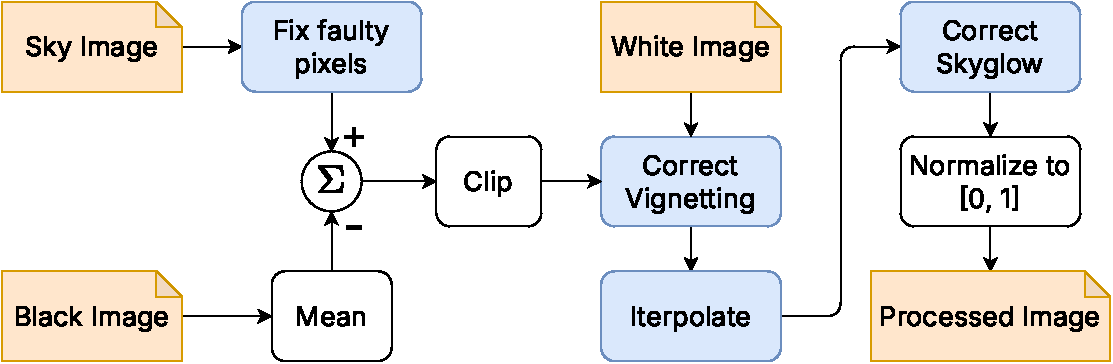
\includegraphics[width=\linewidth]{full_pipeline.pdf}
  \caption{The full pre-processing pipeline for the input image.}
  \label{fig:full-pipeline}
\end{figure}

\begin{figure}[tbp]
  \centering
  \begin{subfigure}{.49\textwidth}
    \centering
    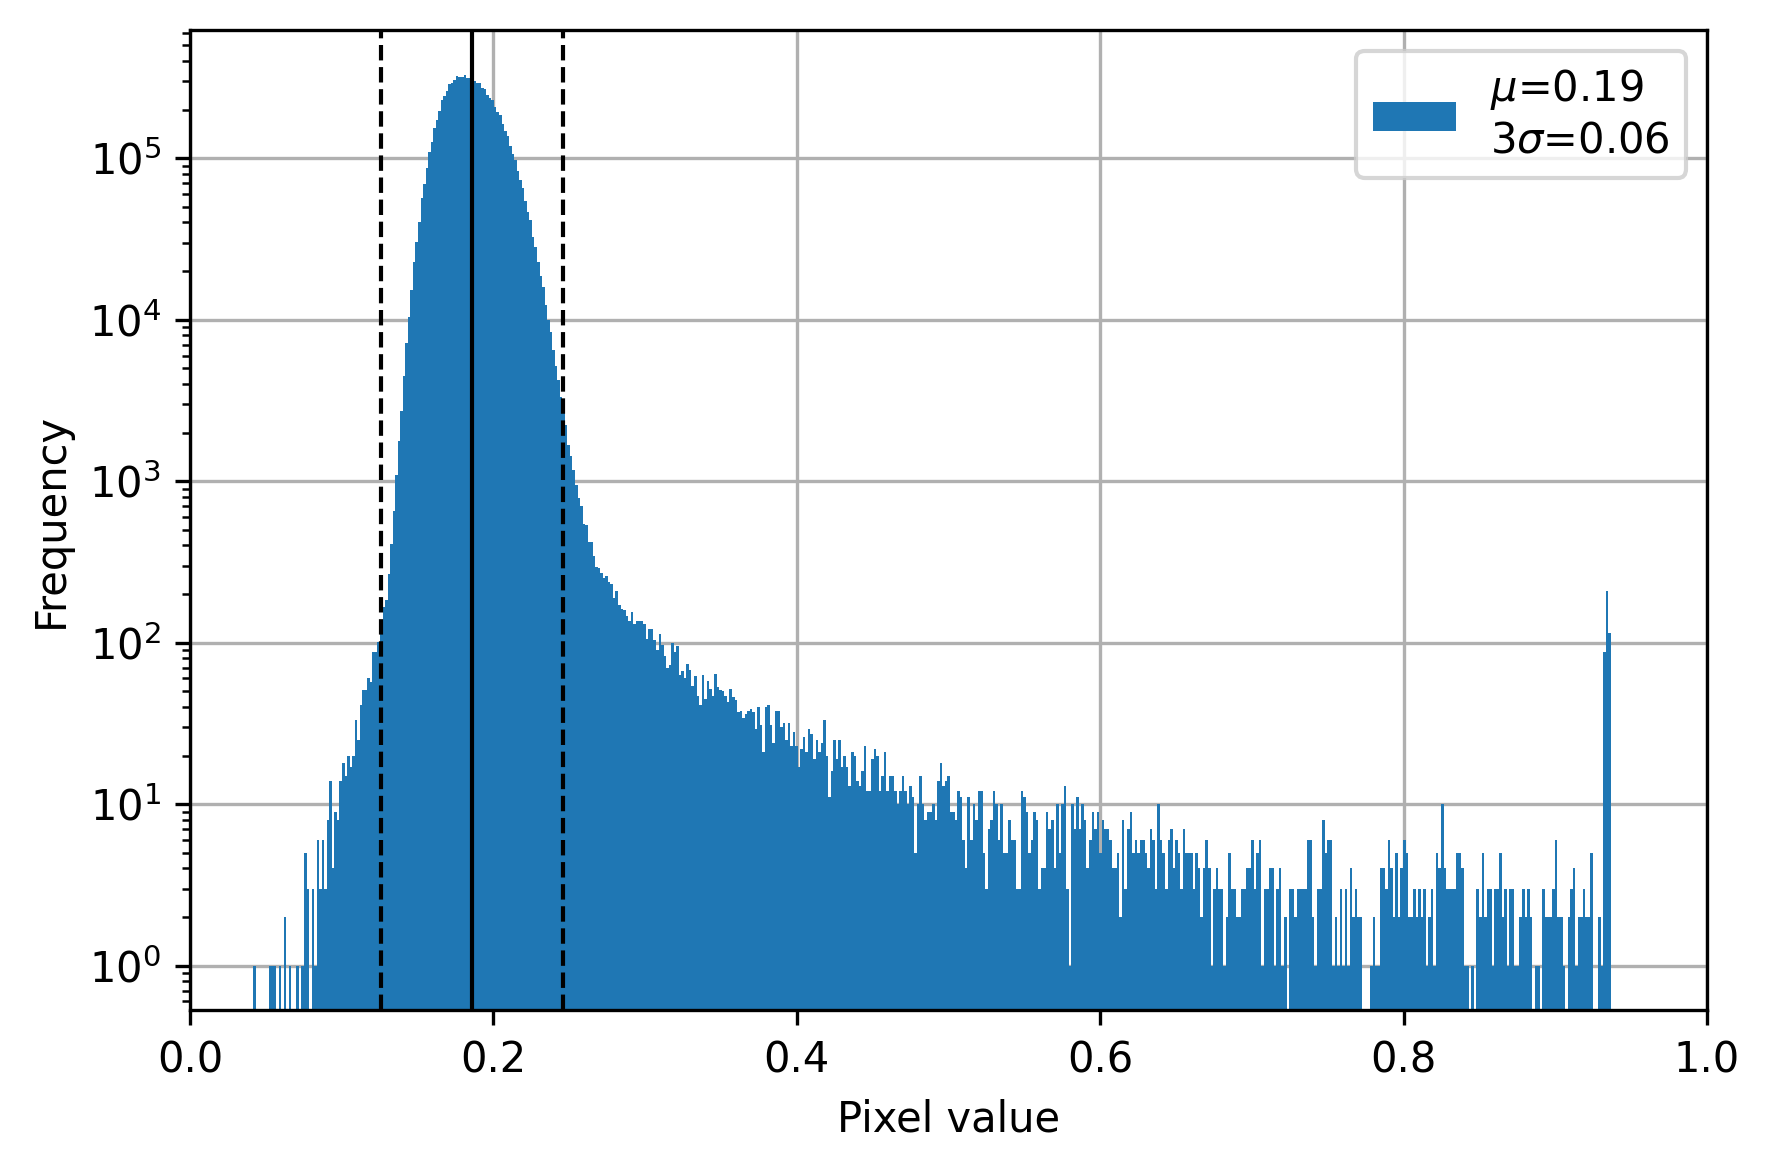
\includegraphics[width=\linewidth]{histogram_input.png}
    \caption{Input image}
    \label{fig:pipeline-input}
  \end{subfigure}%
  \hfill
  \begin{subfigure}{.49\textwidth}
    \centering
    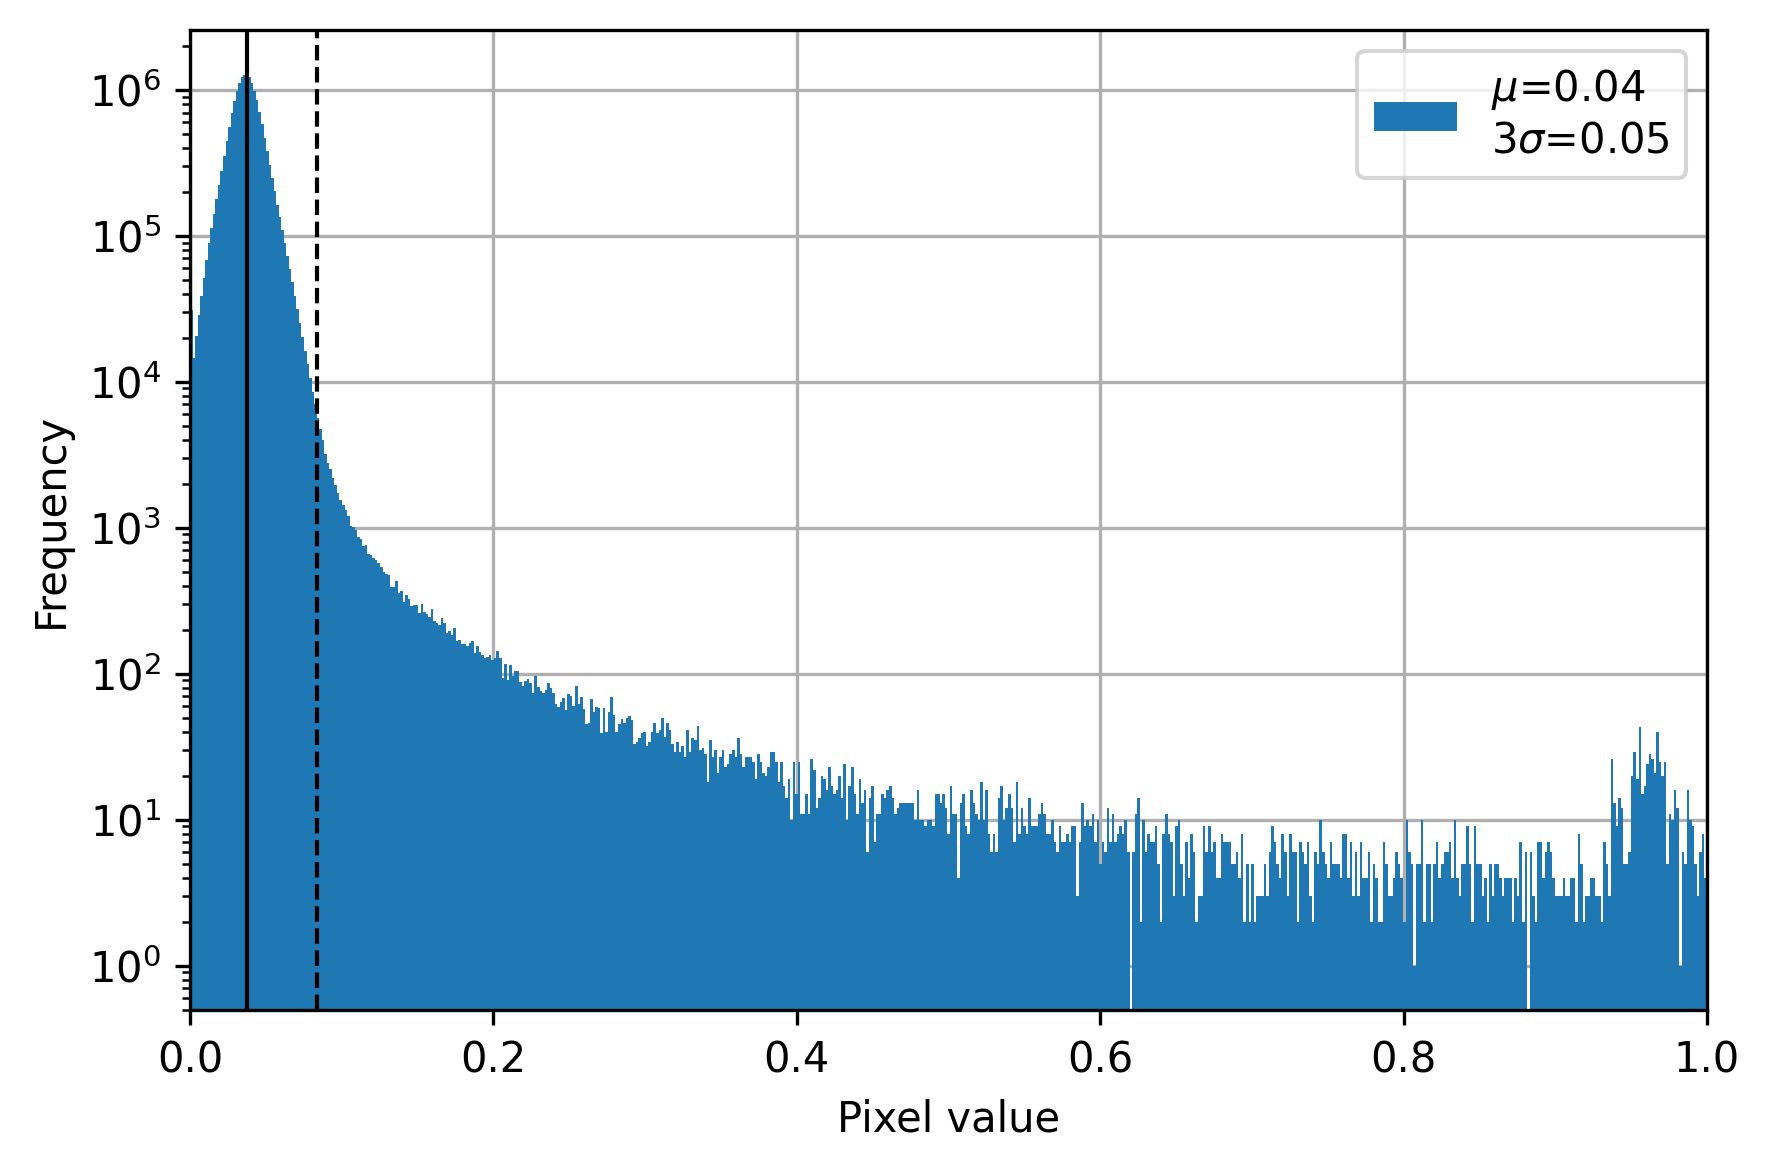
\includegraphics[width=\linewidth]{histogram_output.png}
    \caption{Output image}
    \label{fig:pipeline-output}
  \end{subfigure}
  \caption{Histograms of the input and output images of the full pre-processing pipeline.}
  \label{fig:input-output}
\end{figure}
